\documentclass{beamer}

\usepackage[utf8]{inputenc}
\usepackage{hyperref}

\usetheme{Berkeley}
\beamertemplatenavigationsymbolsempty
\setbeamertemplate{headline}{}
 
\title{Tracing in FoodChain-Lab}
\date{}
 
\begin{document}
\maketitle

\section{Aufgaben}
\begin{frame}
	\begin{itemize}
		\item Nutzen Sie den Beispiel Workflow von \url{https://github.com/SiLeBAT/BfROpenLabResources/raw/master/GitHubPages/workflows/FCL_Example.zip}.
		\item Lassen Sie sich im \textbf{Tracing View} den Forward- und Backward-Trace von einer Station zeigen.
		\item Dann deaktivieren Sie in der schwarzen Station die Kreuzkontamination und schauen Sie, wie sich der Forward Trace daraufhin ändert.
	\end{itemize}
\end{frame}
 
\section{1}
\begin{frame}
	\begin{center}
  		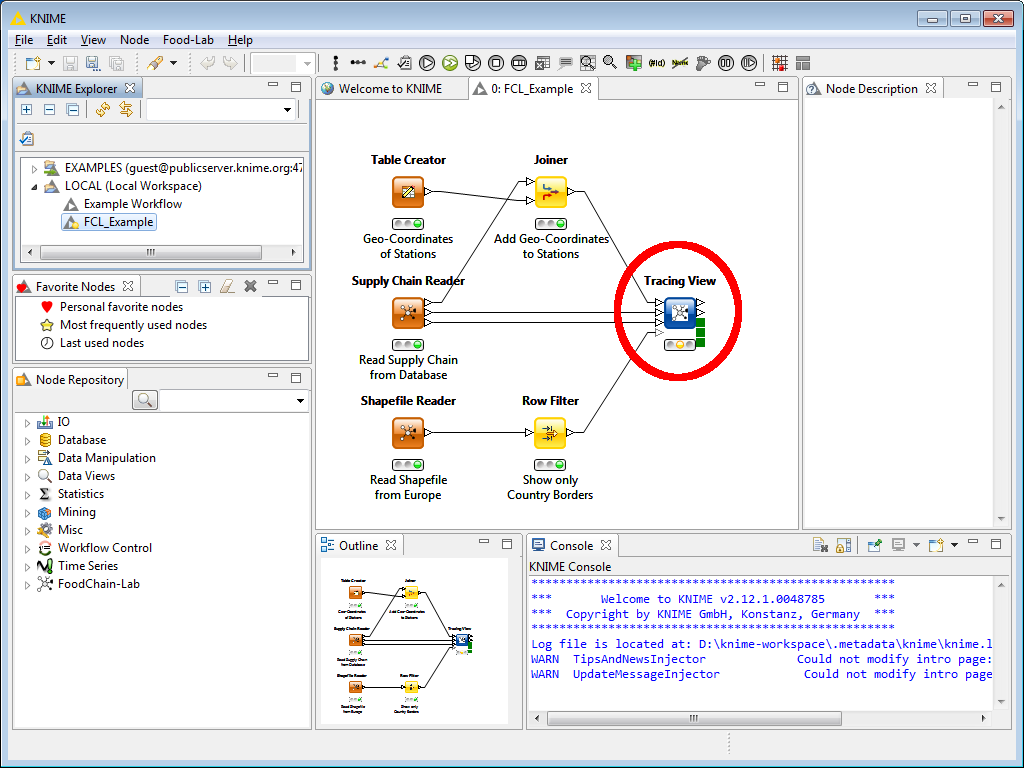
\includegraphics[height=0.6\textheight]{1.png}
	\end{center}
	\begin{itemize}
		\item Importieren Sie den Example Workflow von \url{https://github.com/SiLeBAT/BfROpenLabResources/raw/master/GitHubPages/workflows/FCL_Example.zip}.
		\item Öffnen Sie den \textbf{Tracing View} per Doppelklick.
	\end{itemize}
\end{frame}

\section{2}
\begin{frame}
	\begin{center}
  		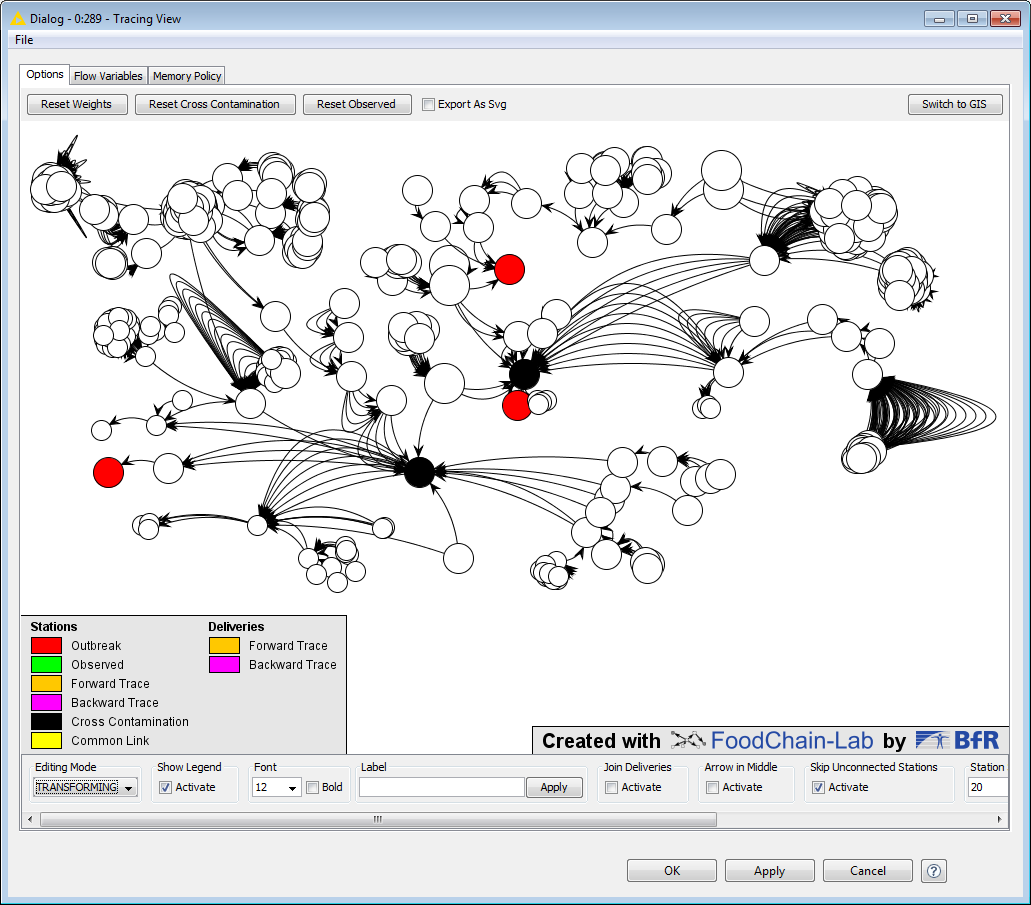
\includegraphics[height=0.6\textheight]{2.png}
	\end{center}
	\begin{itemize}
		\item Im Graphen sehen Sie 9 Ausbruchs-Stationen (rot) and eine Station, an den Kreuzkontamination angenommen wird (schwarz).
		\item Die Größe jeder Station basiert auf ihrem "Score", welcher davon abhängt welche Ausbruchs-Stationen erreicht werden können.
	\end{itemize}
\end{frame}

\section{3}
\begin{frame}
	\begin{center}
  		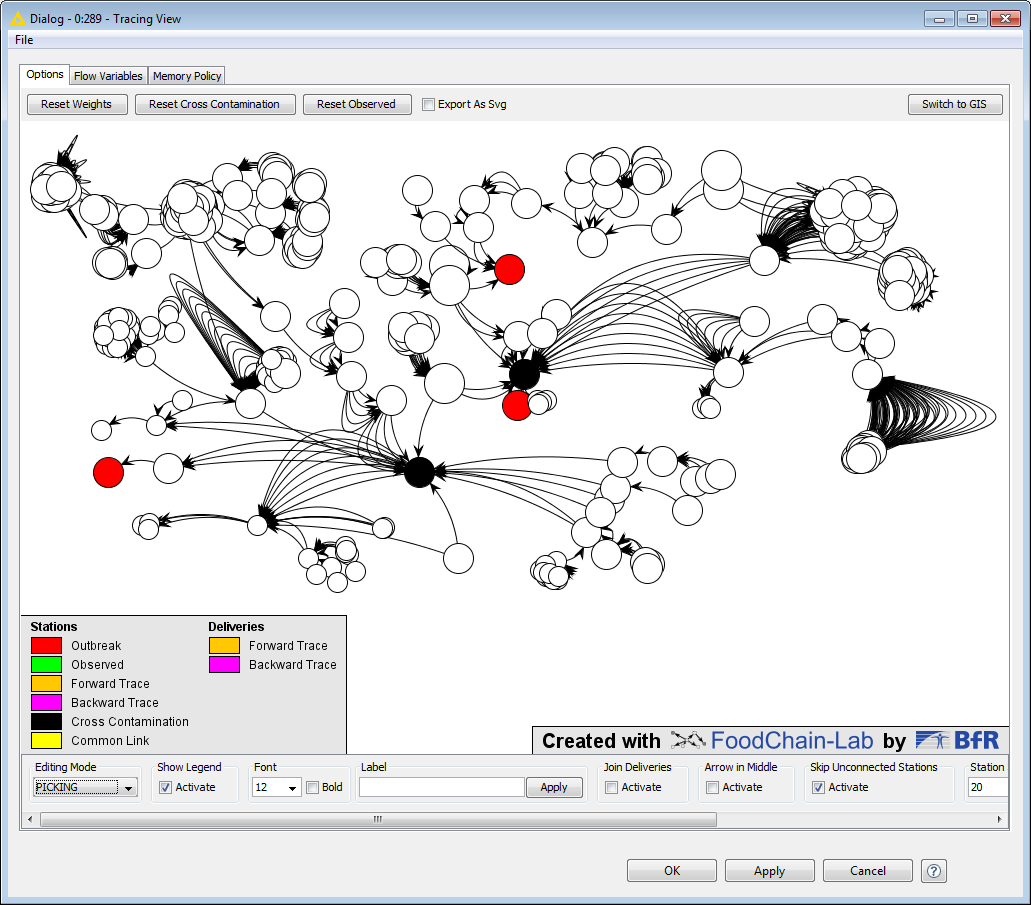
\includegraphics[height=0.6\textheight]{3.png}
	\end{center}
	\begin{itemize}
		\item Wir werden uns nun den Trace einer einzelnen Station im Detail anschauen.
		\item Wählen Sie "Picking" als \textbf{Editing Mode} und machen Sie einen Doppelklick auf die Station im roten Kreis.
	\end{itemize}
\end{frame}

\section{4}
\begin{frame}
	\begin{center}
  		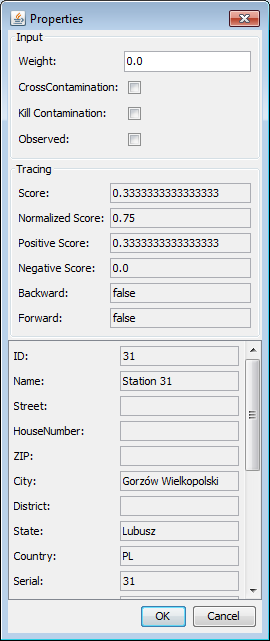
\includegraphics[height=0.6\textheight]{4.png}
	\end{center}
	\begin{itemize}
		\item Ein Dialog mit allen Attributen der ausgewählten Station erscheint.
		\item Im oberen Bereich können Sie die Werte der Attribute "Weight", "CrossContamination", "Kill Contamination" und "Observed" verändern.		
	\end{itemize}
\end{frame}

\section{5}
\begin{frame}
	\begin{center}
  		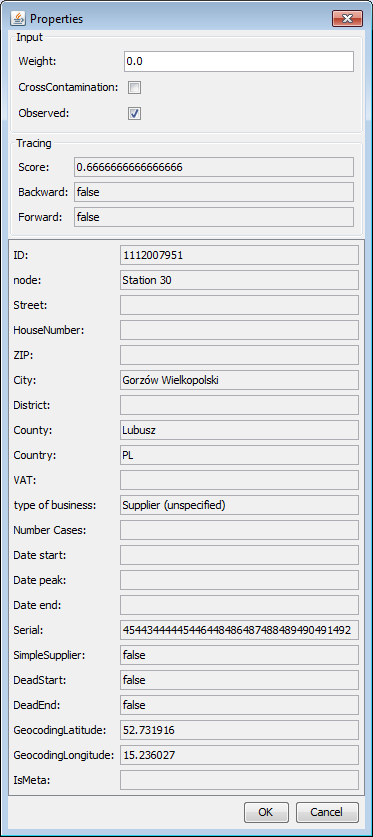
\includegraphics[height=0.6\textheight]{5.png}
	\end{center}
	\begin{itemize}
		\item Aktivieren Sie \textbf{Observed} und drücken Sie \textbf{OK}.
	\end{itemize}
\end{frame}

\section{6}
\begin{frame}
	\begin{center}
  		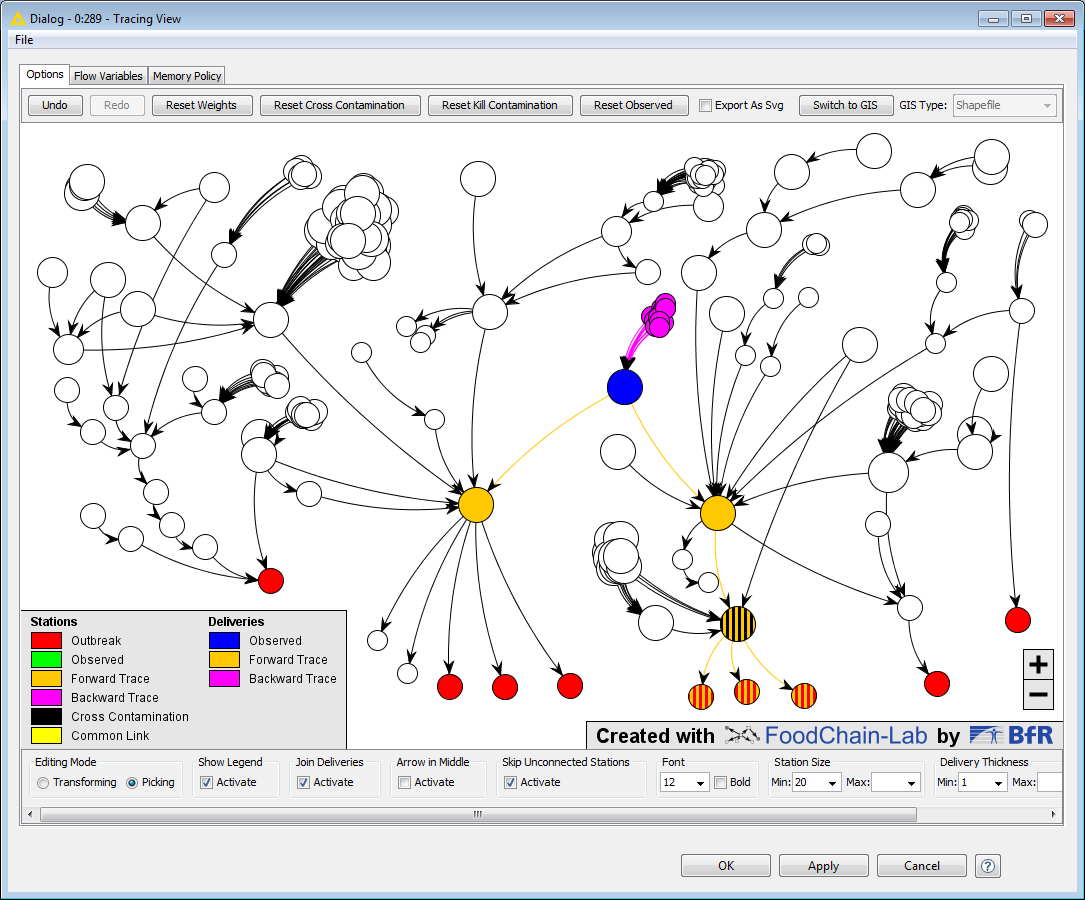
\includegraphics[height=0.6\textheight]{6.png}
	\end{center}
	\begin{itemize}
		\item Alle Stationen/Lieferungen vom Forward-Trace sind orange gefärbt and diejenigen vom Backward-Trace sind magenta.
		\item Drei Ausbruchs-Stationen haben nun orange Streifen. Das bedeutet, dass Sie auch auf dem Forward-Trace sind.
	\end{itemize}
\end{frame}

\section{7}
\begin{frame}
	\begin{center}
  		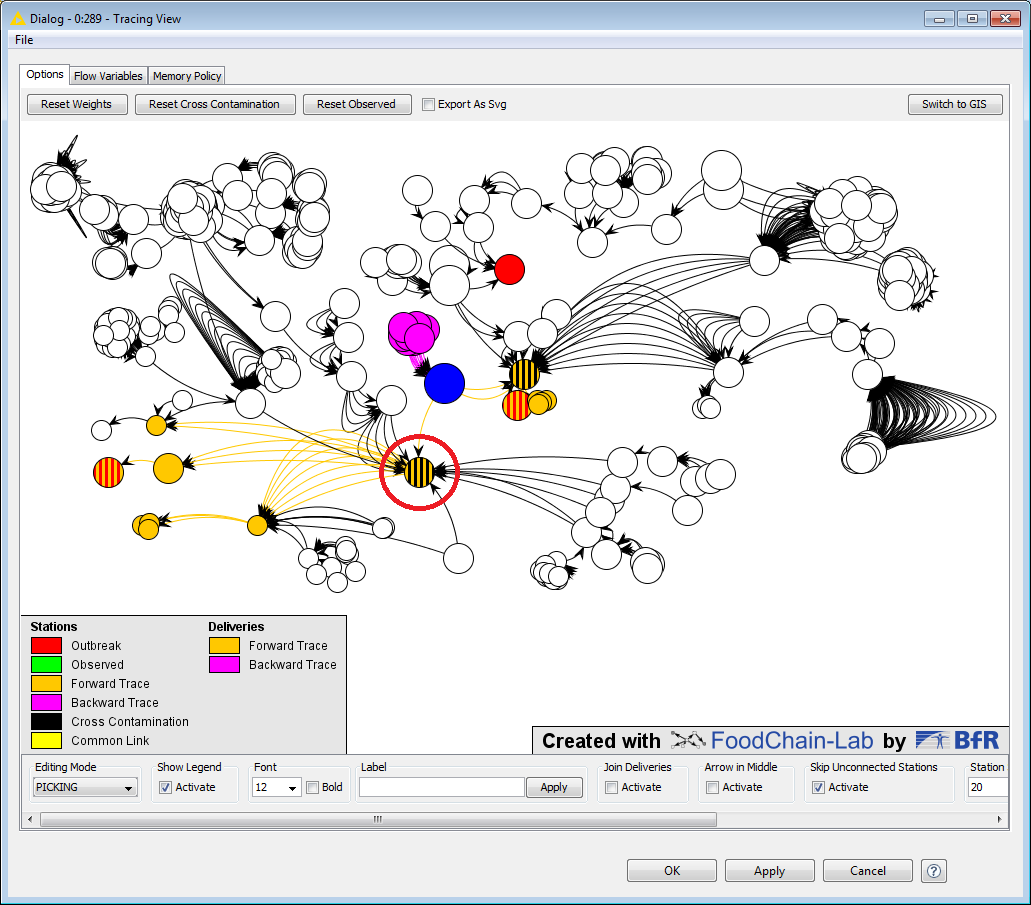
\includegraphics[height=0.6\textheight]{7.png}
	\end{center}
	\begin{itemize}
		\item Nun schauen wir was sich verändert, wenn wir die Kreuzkontamination der Station im roten Kreis deaktivieren.
		\item Machen Sie einen Doppelklick auf die Station.
	\end{itemize}
\end{frame}

\section{8}
\begin{frame}
	\begin{center}
  		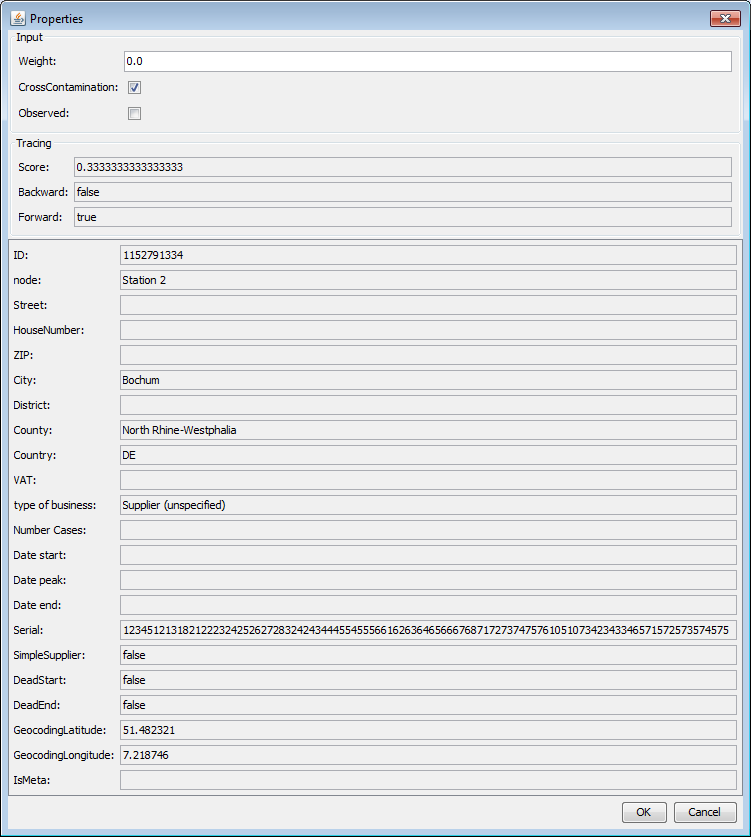
\includegraphics[height=0.6\textheight]{8.png}
	\end{center}
	\begin{itemize}
		\item Deaktivieren Sie \textbf{CrossContamination} und drücken Sie \textbf{OK}.
	\end{itemize}
\end{frame}

\section{9}
\begin{frame}
	\begin{center}
  		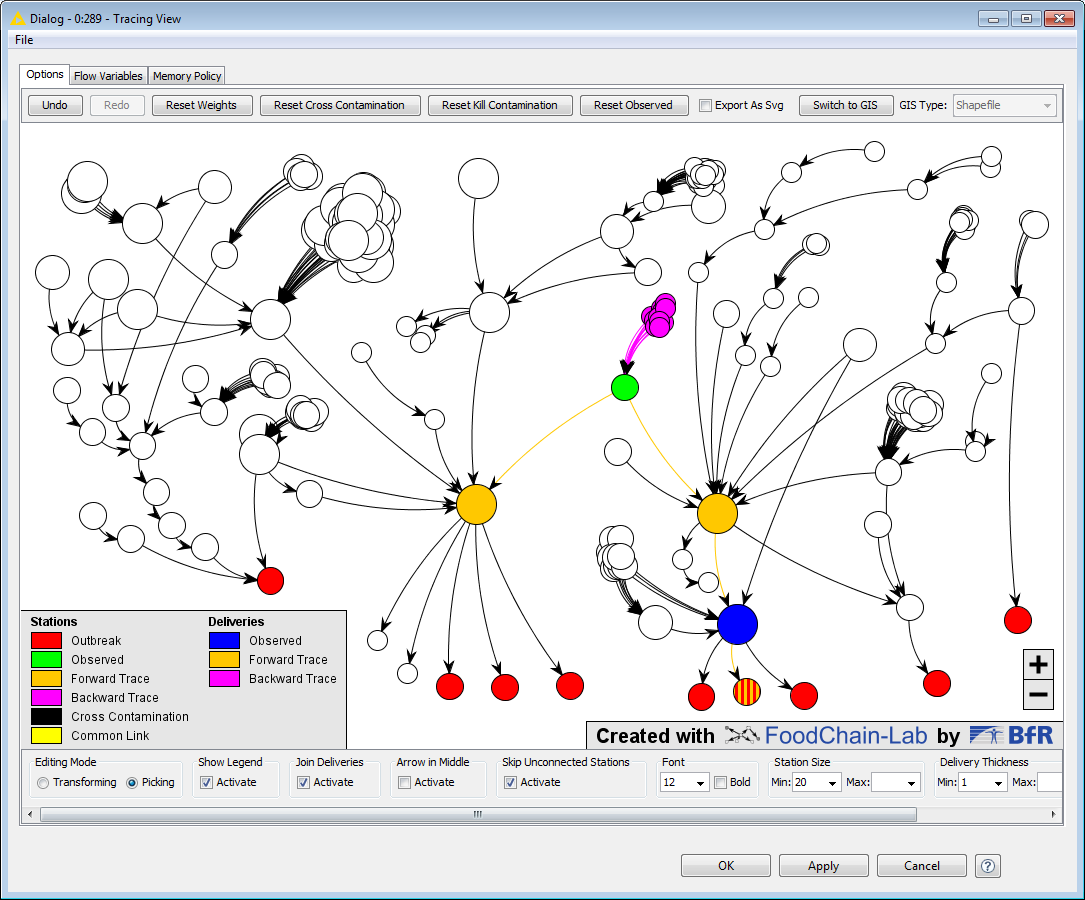
\includegraphics[height=0.6\textheight]{9.png}
	\end{center}
	\begin{itemize}
		\item Das Deaktivieren der Kreuzkontamination hat den Forward-Trace der beobachteten Station ("Observed") verändert.
		\item Nun können zwei Ausbruchs-Stations, die zuvor noch gestreift waren, nicht mehr erreicht werden.
	\end{itemize}
\end{frame}

\end{document}